\documentclass{article}

\usepackage{amsmath,amssymb}
\usepackage{mathtools}
\usepackage{hyperref}
\usepackage{amssymb}
\usepackage{graphicx}
\graphicspath{{../logos/}}


\begin{document}

\setlength{\tabcolsep}{5pt}
\begin{center} \begin{tabular}{cccc}
	
\includegraphics[height=43pt]{SAMF_logo.jpg} &
	
\includegraphics[height=43pt]{SAICA_logo.jpg} &
	
\includegraphics[height=43pt]{OM_Logo_Stacked_Vignette_on_White_RGB.jpg} &
	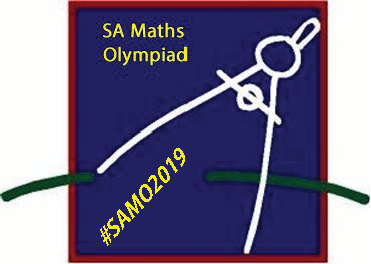
\includegraphics[height=43pt]{SAMO2019.png}
\end{tabular} \end{center}

\bigskip

\begin{center}
\textbf{\Large Another Senior Monthly Problem Set}
\\ \vspace{1em}
\textbf{\large Due: Saturday, 13 June 2020}
\end{center}


\begin{enumerate}

\bigskip
\item[1.] % 2015 Azerbaijan IMO TST Q1, A(N)
A set $A = \{a_1, a_2, \dotsc, a_n\}$ of distinct positive integers is called \emph{powerful} if
\[ \prod_{i \neq j} a_j \mid a_i^{2020} \]
for all $i \in \{1, 2, \dotsc, n\}$.
Find all $n \ge 3$ such that there exists a powerful set containing exactly $n$ elements.


\medskip
\item[2.] % All Russian Olympiad 2017 Grade 10 Q2, G
Let $ABC$ be an acute angled isosceles triangle with $AB = AC$ and circumcentre $O$.
Lines $BO$ and $CO$ intersect $AC$ and $AB$ at $D$ and $E$ respectively.
A straight line $l$ is drawn through $E$ parallel to $AC$.
Prove that the line $l$ is tangent to the circumcircle of $\triangle DOC$.


\medskip
\item[3.] % 2017 Princeton University Maths Competition A4, A
Let the sequence $a_1$, $a_2$, $\dotsc$ be defined by $a_n = 11 a_{n - 1} - n$.
Find the smallest possible value of $a_1$ such that $a_i > 0$ for all $i \in \mathbb{N}$.


\medskip
\item[4.] % China Southeast Math Olympiad 2014, Q2, C
There are $n \ge 4$ people at a fencing competition.
Each player plays against every other player exactly once, and there are no draws.
The organisers decide that the competition is representative if they can find $4$ people, $a_1$, $a_2$, $a_3$, and $a_4$, such that $a_i$ beats $a_j$ whenever $i < j$.
Find the smallest value $n$ such that the competition will always be representative.


\medskip
\item[5.] % 2011 Japan Mathematical Olympiad Finals Problem 5, G
Given some $4$ points in the plane, one can construct $4$ different triangles with vertices amongst the $4$ points.
If the inscribed circles of these $4$ triangles all have the same radius, show that the $4$ triangles are congruent. 


\medskip
\item[6.] % Emile Tredoux 2020, N(G)
Your second favourite thing in this world is Table Mountain, how perfectly horizontal the top of it is.
Your favourite thing in this world is, of course, Mathematics.
Hence, for your birthday you received $n-2$ regular polygons, with number of sides $3, 4, \dotsc, n$ respectively.

You want to combine your two favourite things by stacking all of your polygons on top of each other such that any two consecutively placed polygon share an edge.
For which values of $n$ can you stack your polygon such that the top of your stack is perfectly flat like the top of Table Mountain?
i.e. the top-most edge and bottom-most edge of your stack are parallel.


\medskip
\item[7.] % SAMO Longlist JM-2014-1, N
Let $\mathbb{N}$ denote the set of positive integers.

Consider the function $f : \mathbb{N} \times \mathbb{N} \to \{-1,1\}$, defined as follows:
\[ f(i,j) = \begin{dcases*} -1 & if $i = 1$ or $j = 1$ \\ f(i-1,j) \cdot f(i,j-1) & if $i > 1$ and $j > 1$ \end{dcases*}. \]
Determine the largest $i \leq 2015$ such that $f(i,2015) = -1$.


\medskip
\item[8.] % Moscow Olympiad 1996 59.9.5, C
Ali-Baba and a robber divide a treasure consisting of 100 golden coins, which is initially split into 10 piles of 10 coins each.

Ali-Baba chooses 4 piles, places a mug beside each pile, and puts several coins (at least $1$, but not the whole pile) from the respective pile into each mug.
The robber must permute the mugs, after which the coins are taken out from each mug and added to its newly associated pile.
Then Ali-Baba again selects 4 piles of 10, places mugs beside the piles, etc.

At any moment Ali-Baba can quit and go away with any 3 mugs he chooses, the remaining coins being the robber’s share.
What is the greatest number of coins Ali-Baba can guarantee to collect?

\end{enumerate}


\vfill
\textbf{\Large Email submission guidelines}
\begin{itemize}
	\item Email your solutions to \href{mailto:samf.training.assignments@gmail.com}{\texttt{samf.training.assignments@gmail.com}}.
	\item In the subject of your email, include your name and the level of the assignment (Beginner, Intermediate or Senior).
	\item Submit each question in a single separate PDF file (with multiple pages if necessary), with your name and the question number written on each page.
	\item If you take photographs of your work, use a document scanner such as Office Lens to convert to PDF.
	\item If you have multiple PDF files for a question, combine them using software such as PDFsam.
\end{itemize}

\end{document}
